% !TeX encoding = UTF-8
% !TeX program = xelatex
% !TeX spellcheck = en_US

%********************************************
% whu-proposal: 武汉大学开题报告模版

% Github:https://github.com/whutug/whu-proposal
% Gitee:https://gitee.com/xkwxdyy/whu-proposal
% Update date: 2023-09-26
% Version: v0.8
% Author: Kangwei Xia, kangweixia_xdyy@163.com, School of Mathematics and Statistics, Wuhan University
% QQ group: 681965476
%********************************************


 \documentclass[type = bachelor]{whu-proposal}  % 本科生
% \documentclass[type = master]{whu-proposal}      % 硕士生
%\documentclass[type = doctor]{whu-proposal}      % 博士生


% 个人信息
\ProposalSetup{
  title            = { 纯旋量超弦 } ,
  department       = { 物理科学与技术学院 } ,
  student_id       = { 2021302022016 } ,
  author           = { 郑卜凡 } ,
  % 下面的内容只有【硕|博】需要填写
  major            = { 物理学 } ,
  research_area    = { 弦理论 } , 
  supervisor       = { 杜一剑 } ,
  supervisor_title = { 副教授 } ,
  % year             = { 2023 },  % 年份不填写时默认为编译时的年份
  % month            = { 5 },     % 月份不填写时默认为编译时的月份
  % day              = { 21 },    % 日期不填写时默认为编译时的日期
  show-date = false
}


% 载入所需宏包,下面的仅为示例文件中需要,实际使用时可根据需要增减
% 参考文献
\usepackage[
  backend      = bibtex,
  bibstyle     = gb7714-2015,
  citestyle    = gb7714-2015,
  sorting      = nyt,
  gbnamefmt    = givenahead,
  gbpunctin    = false
]{biblatex}

\addbibresource{whu-proposal.bib}  % 参考文献数据库

\usepackage{amsmath}
\usepackage{amssymb}
\usepackage{graphics}
\usepackage{float}


% 自定义命令,下面的仅为示例文件中需要,实际使用时可根据需要增减
\newcommand\tool{\texttt}
\newcommand\tn[1]{\texttt{\textbackslash#1}}
\newcommand\file{\nolinkurl}
\newcommand\pkg{\textsf}



\begin{document}

% 目录,不需要的话可去除
% \tableofcontents


% 正文内容
\section{选题目的和意义}
自然界四大基本相互作用除引力外已经由粒子物理标准模型很好地描述,其形式框架为量子场论。但是在量子场论的框架下并不能很好地描述量子引力理论,只能将量子引力作为一种有效理论来描述。另外,在量子场论的框架下,标准模型有多达19个自由参数,而且也无法先验地对规范群$SU(3)_C\times SU(2)_L\times U(1)_Y$进行选取。由于量子场论把基本粒子看作是点粒子,所以相互作用都是发生在世界线相交的一个点上,也就是说量子场论具有局域性,这也会导致圈图紫外发散的出现。几乎所有量子场论都必须经过重整化的手段消除圈图发散,而量子引力理论正是一个不可重整化的理论,所以其必定只能是一个某个能标下的有效理论。Weinberg-Witten定理又是局域量子场论和量子引力理论之间矛盾的有力论证\cite{Weinberg:1980kq},这也意味着解决量子引力问题必定需要新的形式理论框架。

弦理论不再把基本粒子看作是点粒子,而是一维延展性的物体——弦。这也意味着相互作用不再是在一个点上进行,而是弥散在世界面相交处的二维面上\cite{Polchinski:1998rq}。而且由于弦理论在世界面上体现为一个二维共形场论,这意味着弦理论有模不变性,这将导致弦理论模空间积分只需要在$SL(2,\mathbb{C})$基本域内积分,而不像量子场论中需要从红外积分到紫外区域,所以弦理论一个显著的特点就是其紫外有限,不需要做重整化\cite{Witten:2015mec}。弦理论另一个诱人的特点在于其理论上并不需要任何额外的参数选取,这意味着如果我们利用弦理论框架构造标准模型讲不会涉及到任何先验的自由度的选取。

弦理论的研究其实起源于强子散射的研究\cite{limiao},Veneziano根据对偶性得到了一个经验公式,并且可以解释为弦之间的散射振幅,但是不久之后量子色动力学(QCD)被确认为强相互作用的模型,弦理论的研究因此也沉寂了很久。直到上个世纪年代,Schwarz、Scherk和Yoneya提议将弦理论看作是一个量子引力理论,弦理论才重新被学术界重视起来。人类研究基本粒子相互作用的唯一途径是通过粒子对撞机,其中的可观测量就是散射振幅。所以散射振幅的计算是量子场论研究中的重要课题。对弦振幅的研究从实用主义的角度来看可以帮助推动量子场论散射振幅的研究。比如量子场论散射振幅计算中极为重要的Kawai-Lawenllen-Tye(KLT)关系\cite{Kawai:1985xq}和Bern-Carrasco-Johansen (BCJ) 关系\cite{Bern:2010ue}都是来源于对弦振幅的分析。另外,从理论框架的角度看,对弦振幅的研究也有利于对弦理论本身的理解。最后,弦理论在数学界也有非常重要的地位,而弦振幅的模空间积分和模形式和黎曼面之间都有很大的联系,而且弦振幅的形式会用到数论中的多对数函数、Multi-Zeta-Values等来描述\cite{Broedel:2014vla},所以弦振幅的研究也能促进对数论的研究\cite{schlottererNumberTheorySuperstring2020}。

早期弦理论主要指玻色弦,但是玻色弦不含费米子态且包含物理上不被允许的快子态。解决此问题的办法是通过引入超对称,这样每一个玻色自由度都对应一个费米自由度,而且快子态也在GSO投影下被消除了\cite{Polchinski:1998rr}。但超对称的引入又涉及到靶空间超对称以及世界面超对称的选择,从超对称的实现上来讲,世界面超对称要容易得多,所以选取世界面超对称的RNS超弦首先得到发展。但是从物理上看我们更需要理论保留靶空间超对称,后面证明RNS超弦中靶空间超对称只是被隐藏起来了,最终计算的结果依旧有靶空间超对称。但是RNS超弦比较适用于靶空间平凡的情况,处理非平凡靶空间中弦的超对称化应当使用保留靶空间超对称的方法。Green和Schwarz最早通过保留靶空间超对称发展了GS超弦,但是最终量子化还是有不少问题。直到本世纪初,Berkovits解决了GS超弦中存在的问题,发展出纯旋量超弦\cite{Berkovits:2000fe}。纯旋量超弦和RNS超弦目前认为在描述超弦理论上是等价的,但是纯旋量超弦在处理非平凡靶空间问题上有显著的优势,特别是有关于弦振幅的计算。更多弦振幅的应用可以见弦微扰论白皮书\cite{berkovits2022snowmasswhitepaperstring}。

本毕业论文主要研究纯旋量超弦在弦振幅计算中的应用,特别是其结果对量子场论散射振幅研究的意义。该选题的主要目的是学习和理解目前学术界有关微扰弦理论方向的重大学术成果,也对理解超对称有很大的意义。

\section{国内外研究现状和发展趋势}
\subsection{国内研究现状和发展趋势}
在微扰量子场论,特别是量子场论散射振幅的研究方向国内目前十分强势。上个世纪徐湛、张达华等人发展的旋量螺旋度方法极大简化了胶子散射振幅的计算,是现代散射振幅在壳技术的起源,被国外同行称为“中国魔术”\cite{Xu:1986xb}。冯波为首的新一代散射振幅研究者发展了幺正切割,BCFW在壳递推关系等当代散射振幅的重要计算工具\cite{Britto:2005fq,Britto:2004ap,Britto:2004nc}。最近十年,何颂、袁野以及Cachazo发展了散射振幅的CHY形式,给予了不同量子场论散射振幅的统一描述框架\cite{Cachazo:2013hca,Cachazo:2013iea}。

但是目前国内对弦振幅的研究还比较落后,很少有专门从事弦振幅研究的人员。特别是纯旋量超弦,目前国内还没有对这一研究的贡献。所以本毕业论文选题对国内弦理论研究而言是比较新颖的研究方向。

\subsection{国外研究现状和发展趋势}
国外目前对纯旋量超弦的研究已经有丰富的成果。比如目前学术界非常关注的AdS/CFT对偶最初是基于$\mathrm{AdS}_5\times \mathcal{S}^5$背景下传播的弦理论,基于纯旋量超弦证明了这个理论在量子层面上的自洽性\cite{Berkovits:2004xu}。量子场论中色运动学对偶中极为重要的BCJ分子也通过纯旋量超弦被成功构造\cite{Mafra:2011kj}。纯旋量超弦和RNS超弦之间的等价性也有不少验证和讨论\cite{Berkovits:2005ng,Berkovits:2024ono}。

与场论振幅按照圈的个数展开不同,弦振幅是按照世界面拓扑(亏格)进行展开的,可以大概地概括为下面的公式:

\begin{equation}
	\mathcal{A}_{\Sigma_g}(\{1,2,\ldots,n\})\sim\int_{\mathcal{M}_{g,n}}\left\langle \left(\begin{array}{c}\text{PCOs and/or}\\\mathrm{b-glosts~\&}\\\text{regulators}\end{array}\right)V_1(z_1)V_2(z_2)\ldots V_n(z_n)\right\rangle_{\Sigma_g}
\end{equation}

所以在弦振幅方面,弦振幅的研究与量子场论振幅研究类似,主要分为模空间被积函数的研究以及积分后的振幅的研究(主要考虑的是在$\alpha'\to0$的极限下)。

\begin{figure}[H]
	\centering
	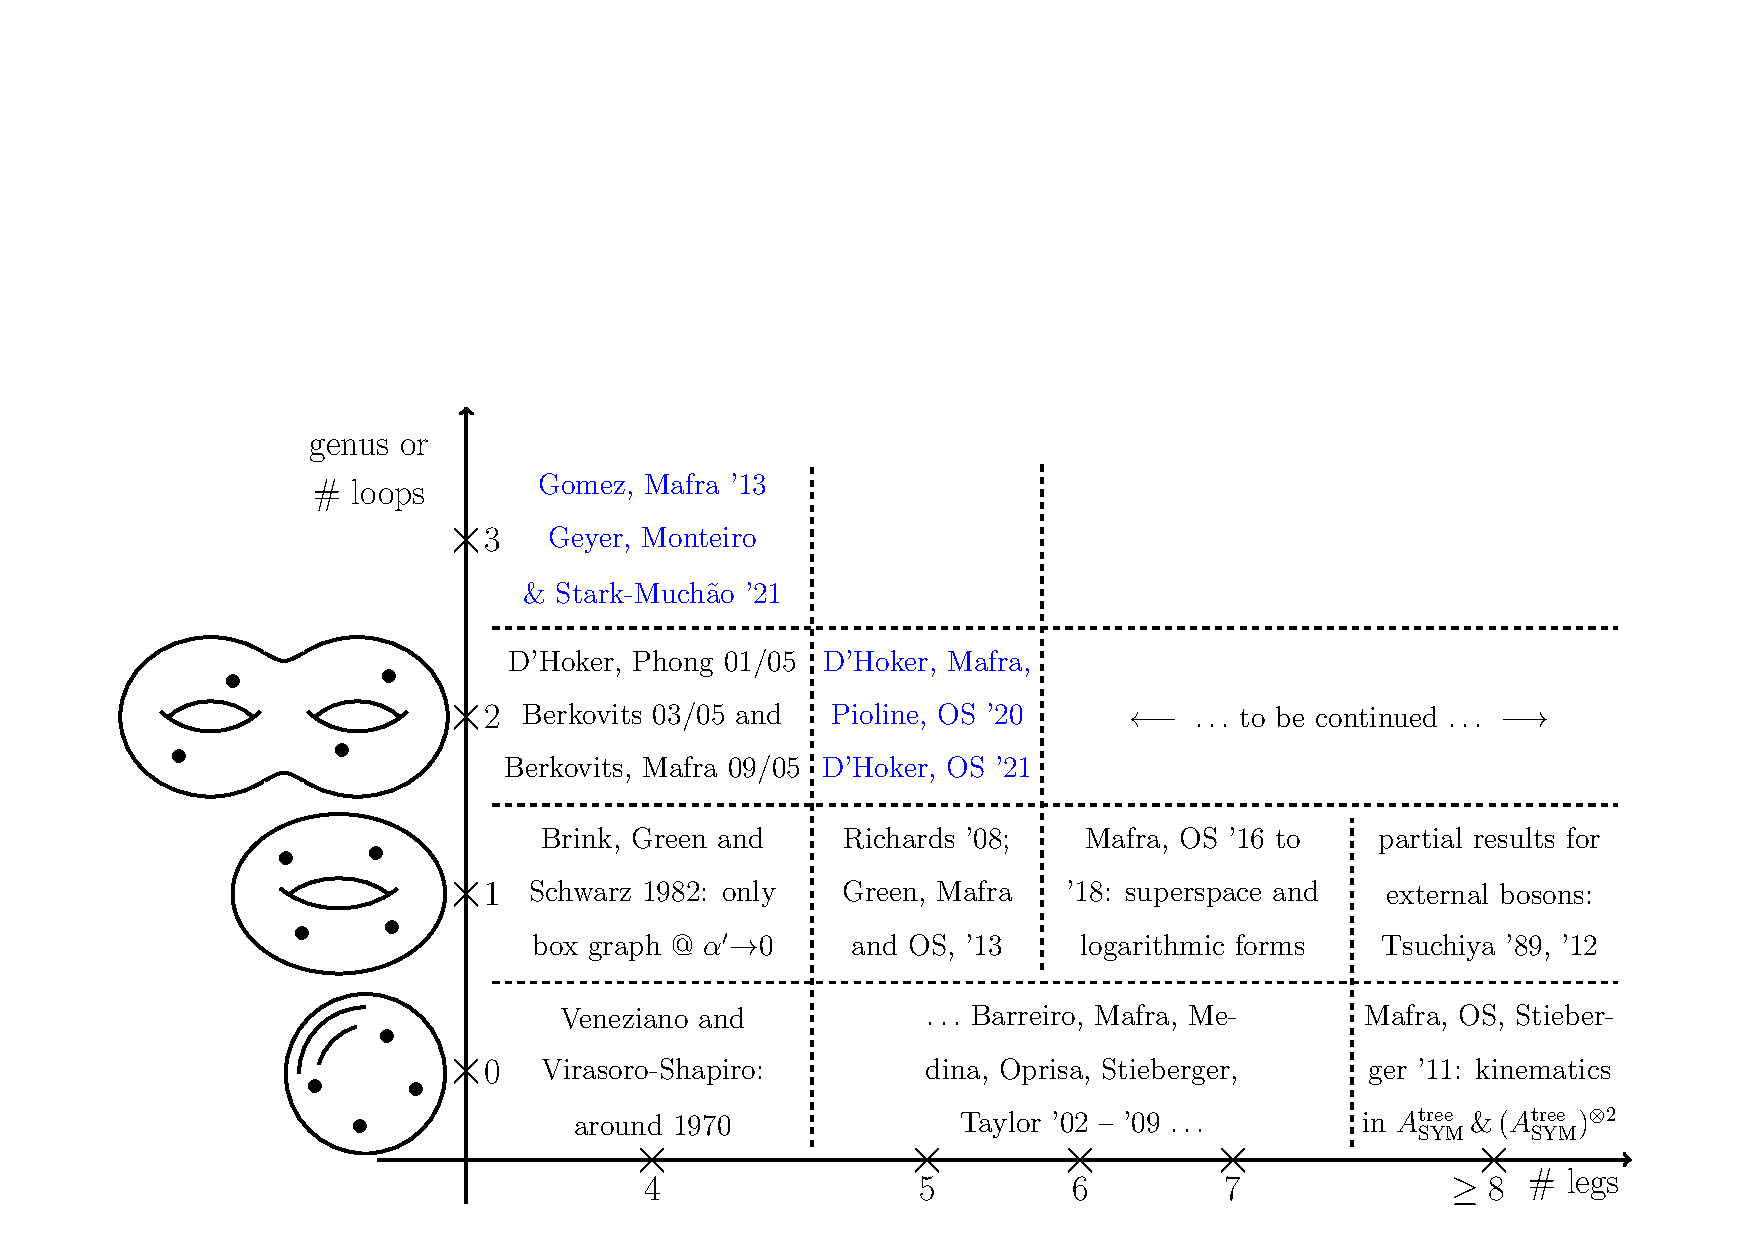
\includegraphics[width=1.0\linewidth]{figures/1.pdf}
	\caption{弦振幅被积函数研究现状}
	\label{fig:1}
\end{figure}

被积函数层面上目前国际上已经有很多研究成果,主要针对的是10维Minkowski时空中的type I / type II超弦的无质量态\cite{Mafra:2011nv,Mafra:2011nw,Geyer:2021oox,Mafra:2022wml,Berkovits:2005df,DHoker:2020tcq,DHoker:2020prr,DHoker:2001kkt},可以概括为图\ref{fig:1}。

另一边,对被积函数积分后会得到大量数论中的结构\cite{Brown:2004ugm,Brown:2011wfj,Broedel:2017jdo},目前的研究大致可以总结为图\ref{fig:2}。

\begin{figure}[H]
	\centering
	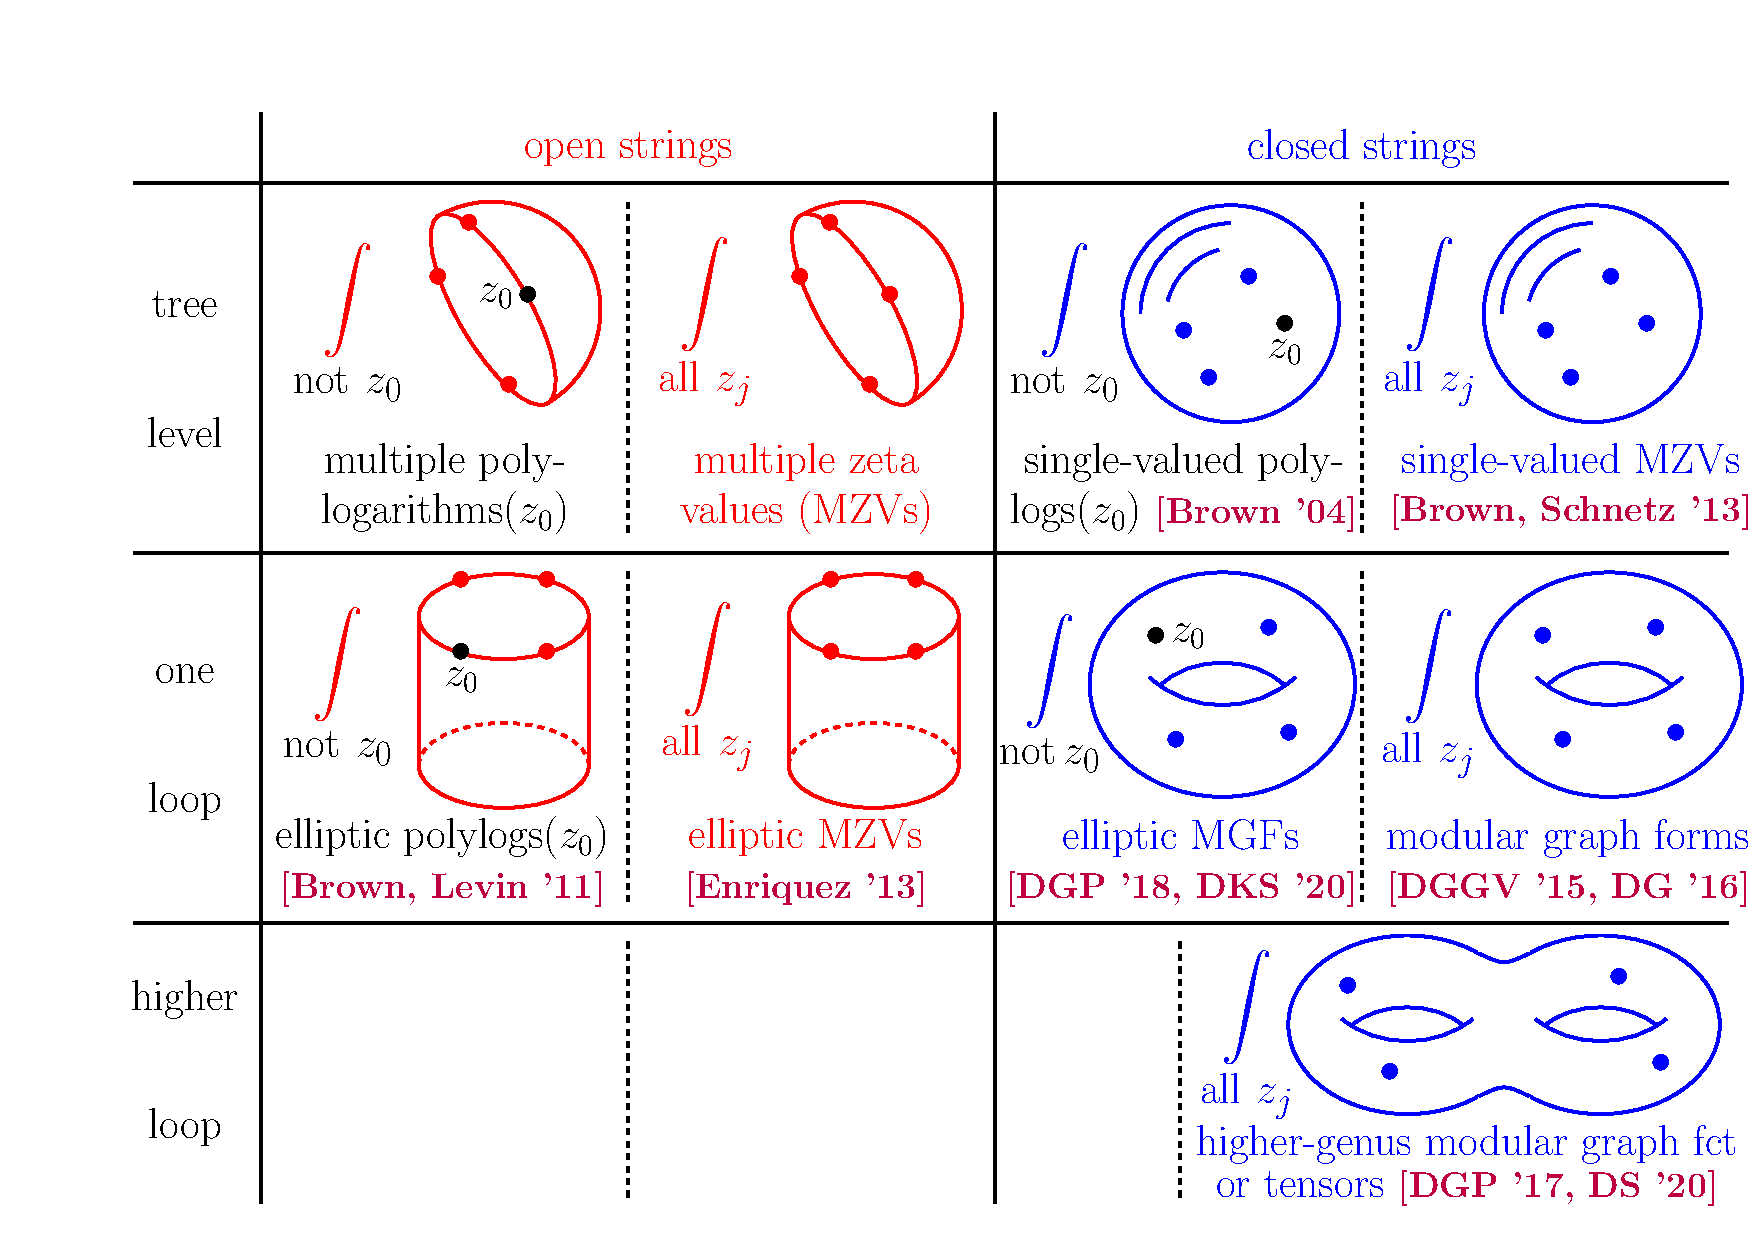
\includegraphics[width=1.0\linewidth]{figures/2.pdf}
	\caption{弦振幅中的数论结构研究}
	\label{fig:2}
\end{figure}

从两幅图中可以直观的看出近年来不断有更高阶的弦振幅计算被解决,随之而来也有更多弦论中的数论结构被发现,而且纯旋量超弦在这些计算中也发挥了很大的作用。所以弦振幅在当今弦理论研究中越来越被重视,特别是由于大型强子对撞机的建设对量子场论标准模型中散射振幅的计算精度有了更大的要求,而弦振幅的发展有利于推动量子场论散射振幅新技术的革命。全息原理、黑洞微观态方面的研究也加大了人们对非平凡靶空间超弦的兴趣。而纯旋量超弦有希望解决这一难题,但是纯旋量超弦发展到目前二十余年,对弦论高激发态顶角算符的构建还存在不少问题亟待解决。总之,弦振幅是目前国际上备受关注的一个话题,纯旋量超弦也有很多重要相关问题有待研究。

\section{研究内容、研究方法、技术路线及可行性分析}
\subsection{研究内容}
Yang-Mills(YM)理论虽然含有四顶点费曼规则,但是总是可以形式上拆分为所有三顶点图的求和,其树级振幅有下面的形式:
\begin{equation}
	A_n^\mathrm{tree}=\sum_{i\in\mathrm{trivalent}}\frac{c_in_i}{\prod_{\alpha_i}p_{\alpha_i}^2}
\end{equation}
这里分母是从图结构可以直接看出来的运动学变量,$c$是顶点带来的色因子,而$n$是最为难从图中直接读出来的项,而且只和外腿运动学变量有关。由于所有图求和的散射振幅才有物理意义,所以单个图的$n$具体为多少并不重要,只要最终求和得到的结果依然是YM理论的散射振幅就是一组合理的选取。但是$c_i$是图结构直接给定的,而且色因子有反对称性和雅可比恒等式,比如图\ref{fig:3}中的三幅费曼图的色因子相加就是0。

\begin{figure}
	\centering
	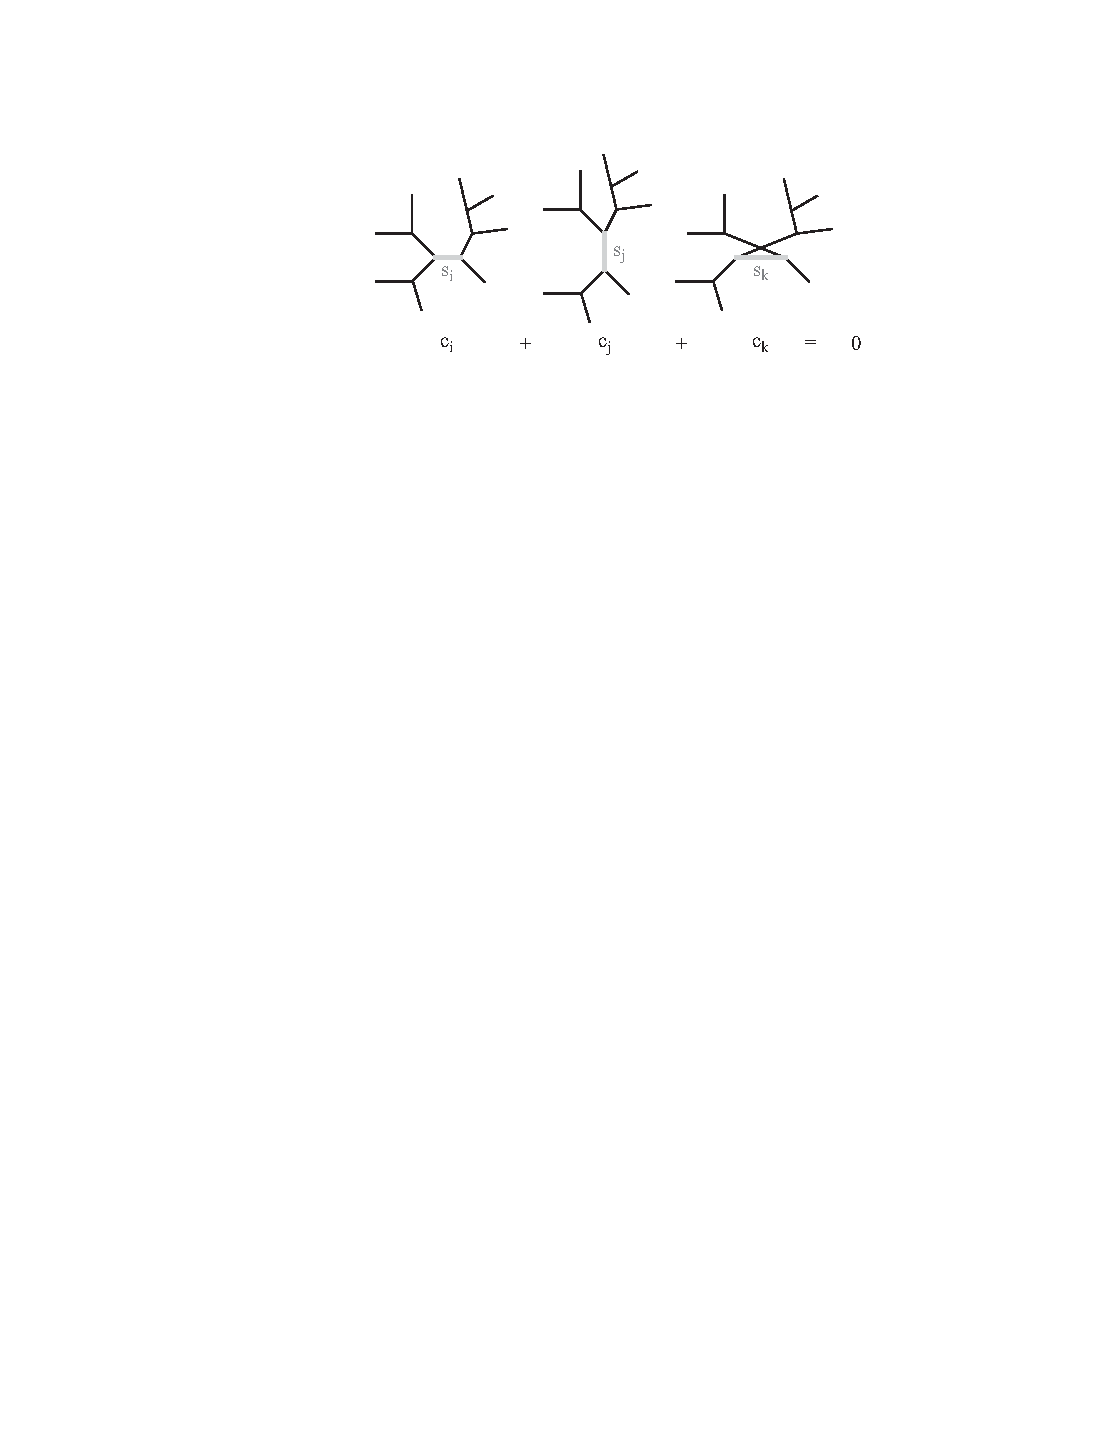
\includegraphics[width=0.85\linewidth]{figures/3.pdf}
	\caption{色因子的雅可比恒等式}
	\label{fig:3}
\end{figure}

那么加入我们能找到一组YM振幅的$n_i$实现,他也满足反对称性和雅可比恒等式:
\begin{equation}
\begin{aligned}
	c_i=-c_j\quad&\Leftrightarrow\quad n_i=-n_j\\
	c_i+c_j+c_k=0\quad&\Leftrightarrow\quad n_i+n_j+n_k=0
\end{aligned}
\end{equation}
那么这组分子我们就叫做BCJ分子,而色运动学对偶(CK对偶)就是说,如果此时将$c_i$全部替换为BCJ分子$n_i$,得到的振幅就是微扰引力振幅:\cite{Elvang:2015rqa}
\begin{equation}
	M_n^\mathrm{tree}=\sum_{i\in\mathrm{cubic}}\frac{n_i^2}{\prod_{\alpha_i}p_{\alpha_i}^2}
\end{equation}
在树图层面上,KLT关系中的动量核就是BCJ分子,所以CK对偶在树级层面是完全正确的,但是圈图层面上还需要更多验证。而且这并不只局限于YM与引力理论之间,比如非线性西格玛模型(NLSM)和特殊伽利略理论(sGal)之间。

虽然BCJ提供了一个非常有用的框架,分析不同理论散射振幅之间的联系,但是BCJ分子的计算非常复杂。Mafra和Oliver等人利用纯旋量超弦计算了树级YM振幅的BCJ因子\cite{Mafra:2011nv},这表明纯旋量超弦在计算BCJ因子上的无限潜力。反过来BCJ因子的计算也能更好地推动弦振幅本身的计算\cite{Geyer:2024oeu}。

本项目主要研究纯旋量超弦在弦振幅计算的应用,以及对YM理论散射振幅BCJ因子构造中的应用。同时本项目也将聚焦数学特别是数论与弦论之间的联系。

\subsection{研究方法}
\begin{itemize}
	\item \textbf{从特殊到一般}
	
	本项目将首先利用纯旋量超弦计算弦振幅,并在$\alpha'\to 0$的极限下分析其与量子场论振幅之间的联系,然后在色基底下进行图展开分析每一项带来的满足条件的BCJ分子。树级振幅的BCJ分子形式比较简单,所以可以用于检验理论的正确性。本项目将从少点树图的计算扩展到高点树图计算并继续尝试对圈图BCJ分子进行一些计算和验证。
	\item \textbf{计算机辅助计算}
	
	纯旋量超弦虽然在形式理论上相较于RNS超弦更适合于非平凡靶空间的弦理论,但是其涉及到大量旋量计算,特别是$\gamma$矩阵的计算。不过目前学术界已经有很多基于\texttt{Mathematica}$^{\textregistered}$或是\texttt{FORM}的旋量计算程序包\cite{Mertig:1990an,Mafra:2010pn}。所以利用这些程序包并开发适用于本项目的计算程序也是本项目的重要研究过程。利用计算机辅助计算可以帮助本项目在研究过程中更关注于物理本质。
\end{itemize}
\subsection{技术路线及可行性分析}
本项目的第一部分将致力于完成弦振幅的计算。树级弦振幅的计算已经有一个成熟的理论框架\cite{Schlotterer:2012zz},并且前述对国内外研究现状的分析也表明,纯旋量超弦散射振幅的计算已有充分的研究基础。

第二部分将从量子场论的角度分析BCJ分子的结构。关于这一方面,已有大量研究成果。例如,基于CHY形式的图展开方法\cite{Du:2017kpo,Fu:2017uzt,Du:2016tbc},以及基于Hopf代数\cite{Brandhuber:2022enp}、自由李代数\cite{Frost:2020eoa}等的多种方法。此外,尽管圈图BCJ因子的计算十分复杂,但已有不少突破性进展,相关综述\cite{Bern:2019prr}对此进行了详细介绍。因此,从量子场论框架下直接分析BCJ分子的结构,已具备了丰富的理论工具。

第三部分将从弦振幅回到量子场论的极限下,基于量子场论振幅的结构直接计算BCJ分子。

最后,本项目还将利用计算机代数系统来辅助计算,特别是基于Mafra的纯旋量计算程序包\cite{Mafra:2010pn},这为完成相关任务提供了有力支持。

综上所述,本项目的技术路线明确且具备良好的逻辑性,具备较强的可操作性。

\section{项目特色与创新点}
本研究项目的特点在于,首先聚焦于纯旋量超弦的理论框架,这一领域目前在国内尚无成熟的研究成果。相比于传统的超弦理论,纯旋量超弦作为一种新的理论形式,具有独特的数学结构和物理背景。具体来说,纯旋量超弦理论不仅有助于弦振幅的计算以及超弦理论的构建,其对量子场论散射振幅计算,特别是在色运动学对偶中的应用,展示了新的潜力。

本项目的创新之处在于,探索纯旋量超弦在色运动学对偶中的具体应用。传统的量子场论散射振幅研究中大多都是局限于量子场论的理论框架下用各种场论中的计算技巧得到BCJ分子。但是本项目基于超弦理论的弦振幅计算,把量子场论散射振幅看作是弦振幅的特定极限。在弦理论这一更高的理论框架下,其振幅会有更多的难以从量子场论本身看出的性质,从而可以更有效的简化计算。这也能够帮助我们更好地理解弦理论与量子场论之间的联系。

通过该研究,旨在推动纯旋量超弦理论的发展,并为量子场论中的散射振幅计算提供新的数学工具与物理意义,进而对高能物理实验中观测到的现象提供理论上的支持与解释。

\section{进度安排}
本项目计划在2024年底之前完成玻色弦及RNS超弦的相关理论学习,并在2025年1月至2月期间深入熟悉超弦的多种形式,进一步扩展对纯旋量超弦的理解。进入2025年3月,计划利用纯旋量超弦框架研究色运动学对偶中的BCJ分子计算,借此更深入地探索量子场论与弦论振幅的数学特性与物理图像。最终,计划于2025年4月集中时间完成毕业论文的撰写,并为毕业答辩做充分准备。

\nocite{*}
\printbibliography[heading=bibintoc,title={六、主要参考文献}]

\end{document}